\noindent Temperature scaling reduces aggregate miscalibration on both datasets but by different amounts. For difficulty-reversed severe, BRACS expected calibration error falls from \num{0.313} to \num{0.067} and negative log likelihood from \num{2.582} to \num{1.271}; on TCGA-UT the same quantities fall from \num{0.140} to \num{0.010} and from \num{1.191} to \num{0.881}. This shows that a large aggregate raw-score difference can reflect correctable confidence scaling, but aggregate repair does not establish repair of the tail-group endpoint.

The aggregate metrics do not substitute for the tail-group endpoint. The contrasts of Section~\ref{sec:rq2-calibration} are therefore re-estimated here on scaled probabilities, holding everything else fixed: the same confirmation runs, the same tail classes taken from each deprived condition's own allocation, the same frozen crossed patient bootstrap, and the same equal-weight average over the three partitions. Recomputing the raw contrasts by the same route reproduces the published values in Tables~\ref{tab:calibration-deficit} and~\ref{tab:calibration-recovery-detail} exactly, which is what licenses reading the scaled column beside them. These scaled contrasts carry paired bootstrap intervals only. The partition-block permutation tests and the Holm adjustment were run on the prespecified raw endpoint and are not repeated here, so no scaled result is a confirmatory decision; the materiality minimum and the interval criterion are applied to them descriptively.

Three findings follow, and they do not point the same way. First, much of the nominal-allocation deficit is removed by adjusting confidence scale. Across BRACS's eight eligible deprived conditions the scaled deficits span $-\num{0.189}$ to \num{0.280} nats; only difficulty-reversed severe, difficulty-reversed severe spread, and difficulty-aligned severe spread still clear the \num{0.148}-nat minimum, and difficulty-aligned moderate, difficulty-aligned severe, and native severe change sign, meaning deprived cross-entropy has lower tail-group NLL than its own balanced reference. TCGA-UT's four eligible nominal conditions behave the same way on a smaller scale: they span $-\num{0.056}$ to \num{0.106} nats, difficulty-aligned severe changes sign, and only the difficulty-aligned and native severe-spread deficits clear its \num{0.061}-nat minimum.

Second, a single confidence adjustment does not remove the independent-support deficit, and this is where the two datasets separate. TCGA-UT's three independent-support deficits fall only from \num{0.258}--\num{0.263} to \num{0.228}--\num{0.232} nats; all three remain above the minimum with intervals excluding zero, so scaling leaves that damage essentially intact. BRACS's equivalents fall from \num{0.134}--\num{0.140} to \num{0.102}--\num{0.109} nats. These positive deficit estimates are reduced, not eliminated, and remain below its \num{0.14782}-nat minimum both before and after scaling. The threshold qualifies the size of the deficit; it does not establish its absence. Holding patch counts fixed while removing patients therefore produces a probability-quality loss that post-hoc calibration does not repair, at the dose where the endpoint is precise enough to read.

Third, the repair credited to prevalence-based weighting does not survive scaling on either dataset, whereas the harm from the other three signals does. On BRACS, \num{14} of the \num{16} raw prevalence-based improvements have intervals excluding zero against one after scaling, and four cells turn into deteriorations. On TCGA-UT the reversal is complete: four raw improvements become none, and all \num{14} scaled cells are deteriorations with intervals excluding zero. The remaining three signals deteriorate throughout: \num{21} of BRACS's \num{24} raw deteriorations qualify and \num{21} of \num{24} scaled ones do, with the largest compressed from \num{2.604} to \num{0.501} nats, while on TCGA-UT \num{18} of \num{21} qualify in both, compressed from \num{0.293} to \num{0.177} nats. Post-hoc calibration therefore undoes much of what the nominal allocation did, and most of what prevalence weighting was credited with repairing, but neither the harm the remaining signals cause nor TCGA-UT's independent-support damage.

\begin{figure}[ht]
  \centering
  \begin{subfigure}[t]{0.48\linewidth}
    \centering
    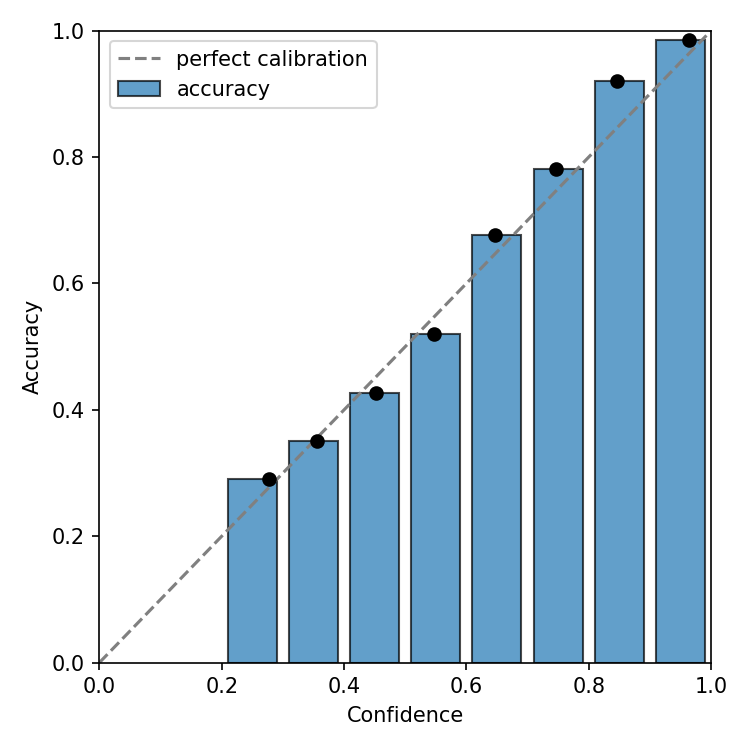
\includegraphics[width=\linewidth]{assets/bracs/reliability_diagram.png}
    \caption{Balanced reference, all classes}
  \end{subfigure}\hfill
  \begin{subfigure}[t]{0.48\linewidth}
    \centering
    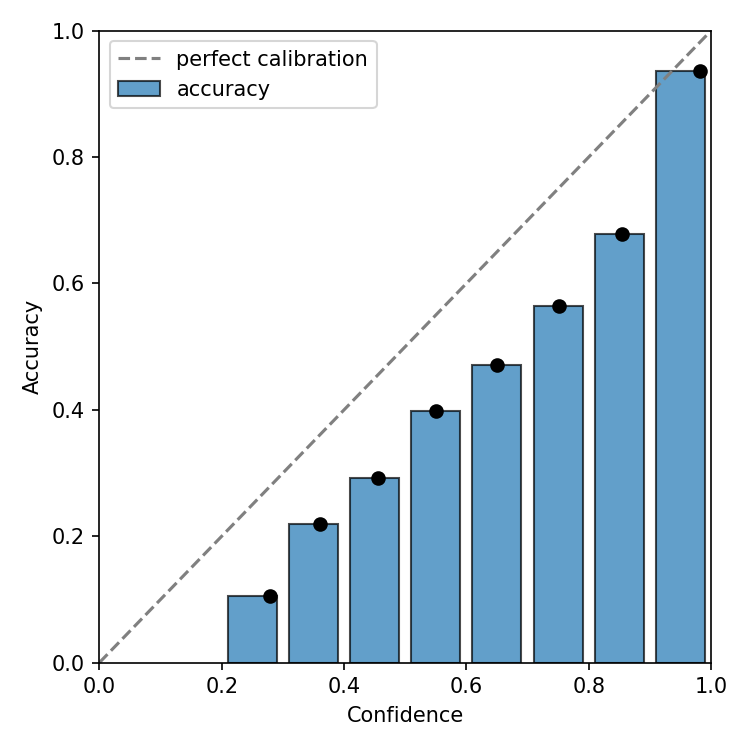
\includegraphics[width=\linewidth]{assets/bracs/tail_reliability_native.png}
    \caption{Severe, native assignment, tail classes}
  \end{subfigure}

  \vspace{0.8em}
  \begin{subfigure}[t]{0.48\linewidth}
    \centering
    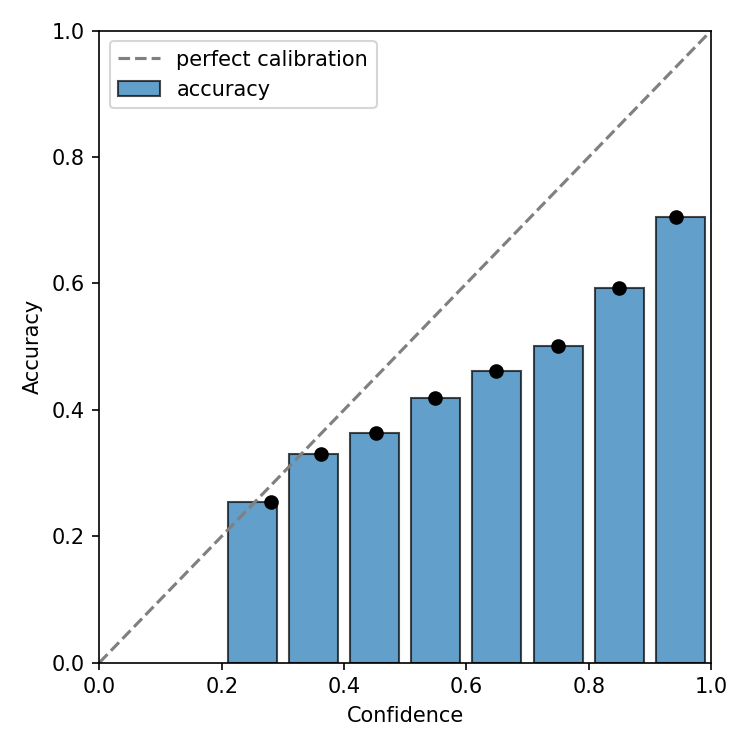
\includegraphics[width=\linewidth]{assets/bracs/tail_reliability_difficulty_aligned.png}
    \caption{Severe, aligned assignment, tail classes}
  \end{subfigure}\hfill
  \begin{subfigure}[t]{0.48\linewidth}
    \centering
    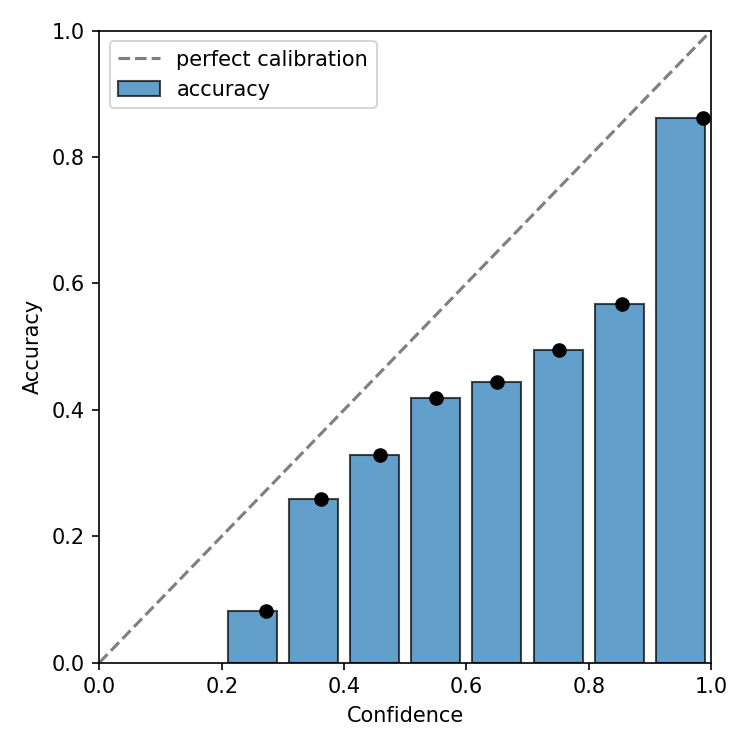
\includegraphics[width=\linewidth]{assets/bracs/tail_reliability_difficulty_reversed.png}
    \caption{Severe, reversed assignment, tail classes}
  \end{subfigure}
  \caption{BRACS reliability curves for the balanced reference and severe-condition tail classes on the first locked partition.}
  \label{fig:reliability-bracs}
\end{figure}

\begin{figure}[ht]
  \centering
  \begin{subfigure}[t]{0.48\linewidth}
    \centering
    
\includegraphics[width=\linewidth]{assets/tcga_ut/reliability_diagram.png}
    \caption{Balanced reference, all classes}
  \end{subfigure}\hfill
  \begin{subfigure}[t]{0.48\linewidth}
    \centering
    
\includegraphics[width=\linewidth]{assets/tcga_ut/tail_reliability_native.png}
    \caption{Severe, native assignment, tail classes}
  \end{subfigure}

  \vspace{0.8em}
  \begin{subfigure}[t]{0.48\linewidth}
    \centering
    
\includegraphics[width=\linewidth]{assets/tcga_ut/tail_reliability_difficulty_aligned.png}
    \caption{Severe, aligned assignment, tail classes}
  \end{subfigure}\hfill
  \begin{subfigure}[t]{0.48\linewidth}
    \centering
    
\includegraphics[width=\linewidth]{assets/tcga_ut/tail_reliability_difficulty_reversed.png}
    \caption{Severe, reversed assignment, tail classes}
  \end{subfigure}
  \caption{TCGA-UT reliability curves for the balanced reference and severe-condition tail classes on the first locked partition. Both figure sets use ten equal-width confidence bins.}
  \label{fig:reliability-tcga}
\end{figure}

